\documentclass[11pt,a4paper]{article}
\usepackage[T1]{fontenc}
\usepackage[utf8]{inputenc}
\usepackage{lmodern}
\usepackage[margin=2.2cm,headheight=14pt]{geometry}
\usepackage{microtype}
\usepackage{amsmath,amssymb,mathtools,bm}
\usepackage{booktabs,tabularx,array}
\usepackage{enumitem}
\usepackage[dvipsnames,table]{xcolor}
\usepackage{tikz}
\usetikzlibrary{arrows.meta,positioning,fit,calc,backgrounds}
\usepackage[most]{tcolorbox}
\usepackage{caption}
\usepackage{adjustbox}
\usepackage{float}
\usepackage{algorithm}
\usepackage{algpseudocode}
\usepackage{fancyhdr}
\usepackage{titlesec}
\usepackage[hidelinks]{hyperref}
\usepackage{xurl}

\definecolor{acc}{HTML}{3F5E44}
\definecolor{ink}{HTML}{1F2933}
\definecolor{gdark}{HTML}{5E7B5F}
\definecolor{glight}{HTML}{E6E9E4}
\definecolor{gbord}{HTML}{4A634B}
\definecolor{rloss}{HTML}{A8323E}
\definecolor{rsoft}{HTML}{F3DCDD}
\definecolor{note}{HTML}{F4F1E8}
\definecolor{bsoft}{HTML}{DCE9F5}
\hypersetup{colorlinks=true,linkcolor=acc,urlcolor=acc,citecolor=acc}

\setlength{\parindent}{0pt}
\setlength{\parskip}{5pt}
\setlist{itemsep=2pt,topsep=3pt}
\titleformat{\section}{\normalfont\Large\bfseries\color{acc}}{\thesection}{0.6em}{}
\titleformat{\subsection}{\normalfont\large\bfseries\color{ink}}{\thesubsection}{0.6em}{}
\pagestyle{fancy}\fancyhf{}
\fancyhead[L]{\small\color{gray}LeFusion: architecture and use for aneurysm CTA}
\fancyhead[R]{\small\color{gray}\nouppercase{\leftmark}}
\fancyfoot[C]{\small\thepage}
\renewcommand{\headrulewidth}{0.3pt}
\captionsetup{font=small,labelfont={bf,color=acc}}

\newtcolorbox{idea}{colback=glight,colframe=gbord,boxrule=0.6pt,arc=2pt,left=6pt,right=6pt,top=4pt,bottom=4pt,fonttitle=\bfseries,title=In one line}
\newtcolorbox{caution}{colback=rsoft!60,colframe=rloss,boxrule=0.6pt,arc=2pt,left=6pt,right=6pt,fonttitle=\bfseries,title=Watch out}
\newtcolorbox{codebox}{colback=note,colframe=gray!60,boxrule=0.4pt,arc=2pt,left=6pt,right=6pt,top=3pt,bottom=3pt,fonttitle=\bfseries\small,title=From the code}

\newcommand{\x}{\bm{x}}
\newcommand{\eps}{\bm{\epsilon}}
\newcommand{\abar}{\bar{\alpha}}
\newcommand{\E}{\mathbb{E}}
\newcommand{\N}{\mathcal{N}}
\newcommand{\Loss}{\mathcal{L}}
\newcommand{\had}{\odot}
\newcommand{\I}{\bm{I}}
\newcommand{\norm}[1]{\left\lVert #1\right\rVert}

\tikzset{
  dk/.style={draw=gbord,fill=gdark,text=white,rounded corners=3pt,align=center,font=\small,minimum height=11mm,minimum width=28mm,inner sep=4pt},
  lt/.style={draw=gray!60,fill=glight,text=black,rounded corners=3pt,align=center,font=\small,minimum height=11mm,minimum width=28mm,inner sep=4pt},
  bl/.style={draw=gray!60,fill=bsoft,text=black,rounded corners=3pt,align=center,font=\small,minimum height=9mm,minimum width=22mm,inner sep=3pt},
  ls/.style={draw=rloss,fill=rsoft,text=black,rounded corners=3pt,align=center,font=\small,minimum height=11mm,minimum width=28mm,inner sep=4pt,line width=0.8pt},
  nt/.style={draw=gray!50,fill=note,text=black!80,rounded corners=3pt,align=left,font=\footnotesize,inner sep=5pt},
  ar/.style={-{Stealth[length=2.4mm]},line width=0.8pt,draw=black!75},
  ard/.style={-{Stealth[length=2.4mm]},line width=0.8pt,draw=rloss,dashed},
  lb/.style={font=\footnotesize\itshape,text=black!70,align=center},
  frame/.style={draw=gbord,rounded corners=6pt,dashed,line width=0.7pt,inner sep=6pt},
}
\begin{document}

\begin{center}
{\LARGE\bfseries\color{ink} LeFusion: Architecture and How We Use It}\\[6pt]
{\large Inserting aneurysms into real CTA patches}\\[6pt]
{\small Prepared for Charitha \quad$\cdot$\quad November 2026}
\end{center}

\begin{idea}
LeFusion is a 3D diffusion model that learns to draw \emph{only the lesion} inside a mask. When generating, everything outside the mask is taken from a real scan, so the background stays real and the mask is exact.
\end{idea}

\textbf{Paper:} H.~Zhang \emph{et al.}, ``LeFusion: Controllable Pathology Synthesis via Lesion-Focused Diffusion Models'', ICLR 2025~\cite{lefusion}.
\textbf{Code} (Apache-2.0): \url{https://github.com/HINTLab/LeFusion}.
All details below were checked against the released code. Where the paper says something different, Section~\ref{sec:diff} lists it.

\tableofcontents

% =====================================================
\section{What LeFusion does}
\begin{itemize}
  \item \textbf{Training:} take real lesion patches, add noise, and teach the network to predict that noise. The error is counted \emph{only inside the lesion mask}.
  \item \textbf{Generation:} take a \emph{normal} patch, a mask and a histogram. Start from noise. At every step, the network draws the lesion, and the area outside the mask is replaced by the real normal patch.
\end{itemize}

\begin{figure}[H]
\centering
\begin{adjustbox}{max width=\linewidth}
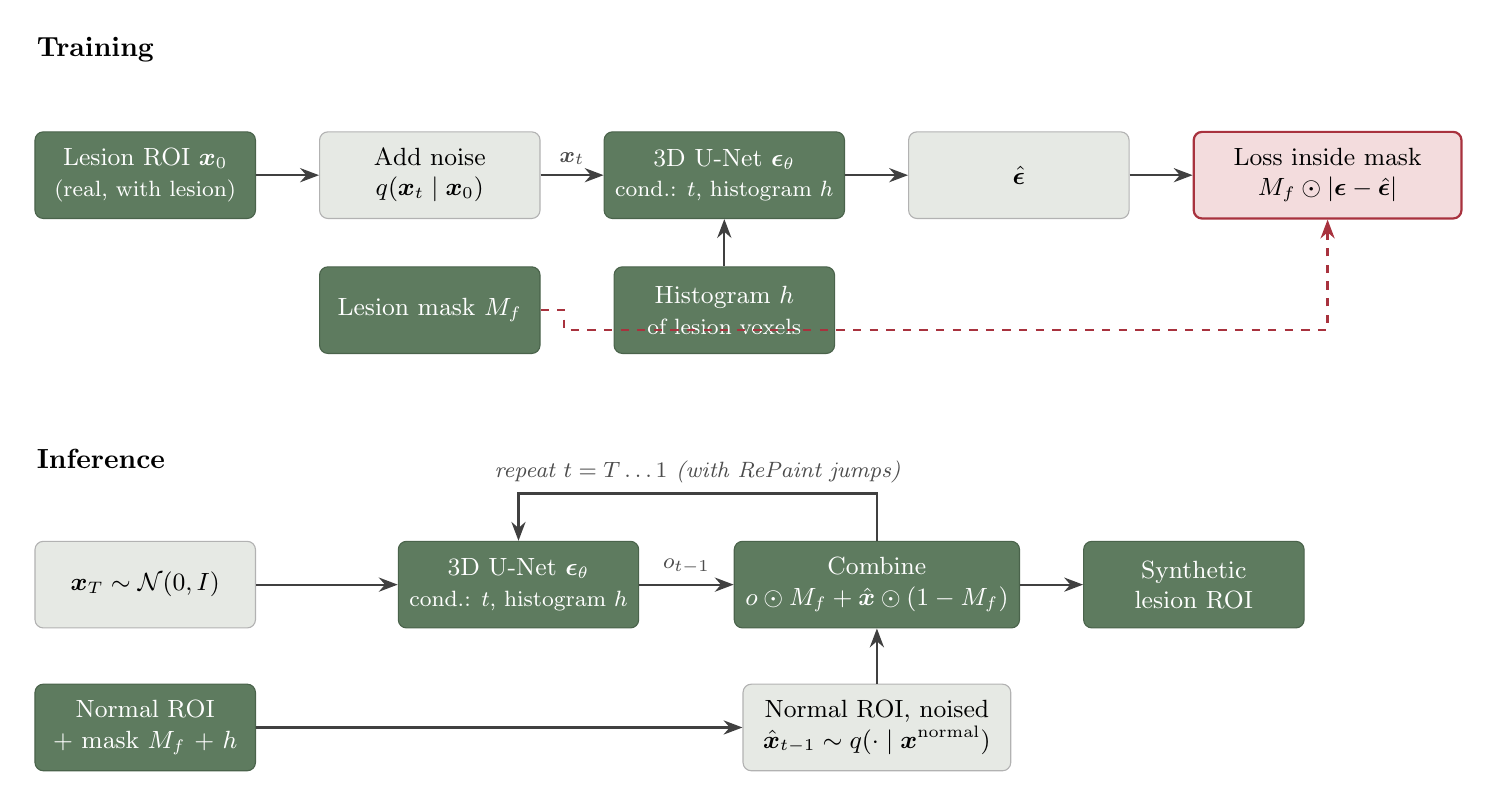
\begin{tikzpicture}[node distance=7mm and 8mm]
% training row
\node[font=\bfseries, anchor=west] at (-1.5,1.6) {Training};
\node[dk] (x0) at (0,0) {Lesion ROI $\x_0$\\\footnotesize (real, with lesion)};
\node[lt, right=of x0] (q) {Add noise\\$q(\x_t\mid\x_0)$};
\node[dk, right=of q, minimum width=30mm] (u1) {3D U-Net $\eps_\theta$\\\footnotesize cond.: $t$, histogram $h$};
\node[lt, right=of u1] (e1) {$\hat\eps$};
\node[ls, right=of e1, minimum width=34mm] (l1) {Loss inside mask\\$M_f\odot|\eps-\hat\eps|$};
\node[dk, below=6mm of q] (m1) {Lesion mask $M_f$};
\node[dk, below=6mm of u1] (h1) {Histogram $h$\\\footnotesize of lesion voxels};
\draw[ar] (x0)--(q); \draw[ar] (q)--node[lb,above]{$\x_t$}(u1); \draw[ar] (u1)--(e1); \draw[ar] (e1)--(l1);
\draw[ar] (h1)--(u1);
\draw[ard] (m1.east) -- ++(3mm,0) |- ([yshift=-14mm]l1.south) -- (l1.south);
% inference row
\node[font=\bfseries, anchor=west] at (-1.5,-3.6) {Inference};
\node[lt] (xT) at (0,-5.2) {$\x_T\sim\N(0,I)$};
\node[dk, right=of xT, xshift=10mm, minimum width=30mm] (u2) {3D U-Net $\eps_\theta$\\\footnotesize cond.: $t$, histogram $h$};
\node[dk, right=12mm of u2, minimum width=34mm] (cb) {Combine\\$o\odot M_f+\hat\x\odot(1-M_f)$};
\node[lt, below=7mm of cb, minimum width=34mm] (bg) {Normal ROI, noised\\$\hat\x_{t-1}\sim q(\cdot\mid\x^{\text{normal}})$};
\node[dk, right=of cb] (out) {Synthetic\\lesion ROI};
\node[dk, below=7mm of xT] (n) {Normal ROI\\+ mask $M_f$ + $h$};
\draw[ar] (xT)--(u2); \draw[ar] (u2)--node[lb,above]{$o_{t-1}$}(cb); \draw[ar] (bg)--(cb); \draw[ar] (cb)--(out);
\draw[ar] (n.east) -- (bg.west);
\draw[ar] (cb.north) |- ++(0,6mm) -| node[lb,pos=0.25,above]{repeat $t=T\dots1$ (with RePaint jumps)} (u2.north);
\end{tikzpicture}
\end{adjustbox}
\caption{LeFusion overview (redrawn from the paper's framework figure). Top: training uses only real lesion ROIs and a lesion-focused loss. Bottom: inference keeps the real normal background and generates only inside $M_f$.}
\label{fig:overview}
\end{figure}


% =====================================================
\section{The network}

\subsection{3D U-Net}
The network is a ``video-style'' 3D U-Net. It treats depth like time in a video: it works inside each slice and across slices separately.

\begin{figure}[H]
\centering
\begin{adjustbox}{max width=\linewidth}
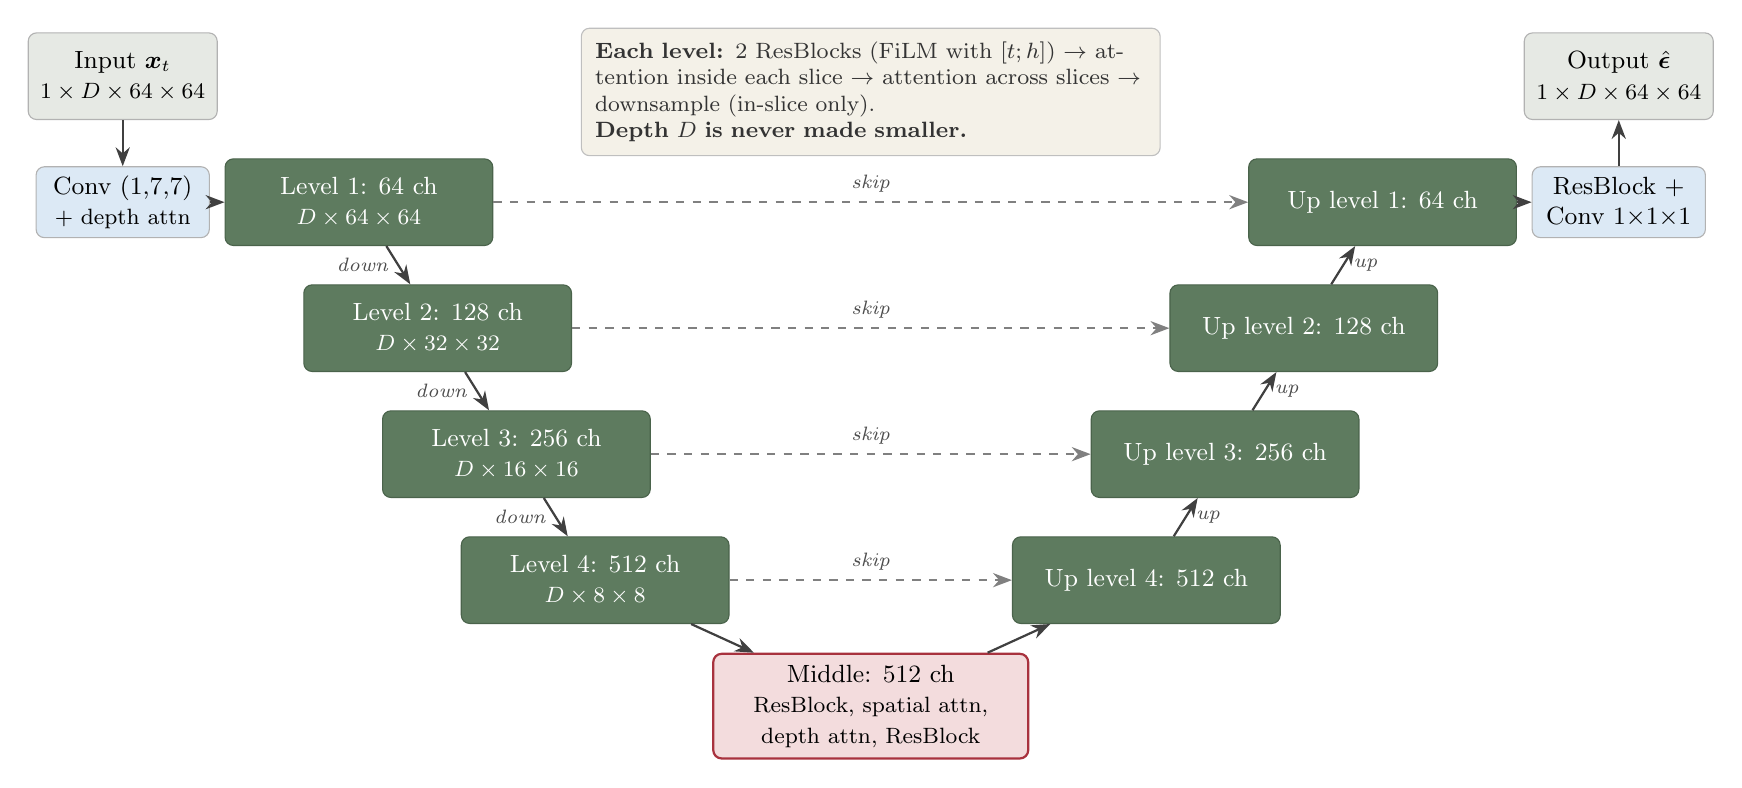
\begin{tikzpicture}[x=1mm,y=1mm]
% encoder
\node[lt, minimum width=24mm] (in) at (0,0) {Input $\x_t$\\\footnotesize $1\times D\times64\times64$};
\node[bl] (c0) at (0,-16) {Conv $(1{,}7{,}7)$\\\footnotesize + depth attn};
\node[dk, minimum width=34mm] (e1) at (30,-16) {Level 1: 64 ch\\\footnotesize $D\times64\times64$};
\node[dk, minimum width=34mm] (e2) at (40,-32) {Level 2: 128 ch\\\footnotesize $D\times32\times32$};
\node[dk, minimum width=34mm] (e3) at (50,-48) {Level 3: 256 ch\\\footnotesize $D\times16\times16$};
\node[dk, minimum width=34mm] (e4) at (60,-64) {Level 4: 512 ch\\\footnotesize $D\times8\times8$};
\node[ls, minimum width=40mm] (mid) at (95,-80) {Middle: 512 ch\\\footnotesize ResBlock, spatial attn,\\\footnotesize depth attn, ResBlock};
\node[dk, minimum width=34mm] (d4) at (130,-64) {Up level 4: 512 ch};
\node[dk, minimum width=34mm] (d3) at (140,-48) {Up level 3: 256 ch};
\node[dk, minimum width=34mm] (d2) at (150,-32) {Up level 2: 128 ch};
\node[dk, minimum width=34mm] (d1) at (160,-16) {Up level 1: 64 ch};
\node[bl] (cf) at (190,-16) {ResBlock +\\Conv $1{\times}1{\times}1$};
\node[lt, minimum width=24mm] (out) at (190,0) {Output $\hat\eps$\\\footnotesize $1\times D\times64\times64$};
\draw[ar] (in)--(c0); \draw[ar] (c0)--(e1);
\draw[ar] (e1)--node[lb,left]{\scriptsize down}(e2); \draw[ar] (e2)--node[lb,left]{\scriptsize down}(e3); \draw[ar] (e3)--node[lb,left]{\scriptsize down}(e4);
\draw[ar] (e4)--(mid); \draw[ar] (mid)--(d4);
\draw[ar] (d4)--node[lb,right]{\scriptsize up}(d3); \draw[ar] (d3)--node[lb,right]{\scriptsize up}(d2); \draw[ar] (d2)--node[lb,right]{\scriptsize up}(d1);
\draw[ar] (d1)--(cf); \draw[ar] (cf)--(out);
\foreach \a/\b in {e1/d1,e2/d2,e3/d3,e4/d4} \draw[ar, dashed, draw=gray] (\a)--node[lb,above]{\scriptsize skip}(\b);
\node[nt, text width=70mm] at (95,-2) {\textbf{Each level:} 2 ResBlocks (FiLM with $[t;h]$) $\rightarrow$ attention inside each slice $\rightarrow$ attention across slices $\rightarrow$ downsample (in-slice only).\\\textbf{Depth $D$ is never made smaller.}};
\end{tikzpicture}
\end{adjustbox}
\caption{Denoising U-Net of LeFusion [code]: base width 64, channel multipliers $(1,2,4,8)$, four levels. Down- and up-sampling act only on the in-slice size; the depth stays the same through the whole network.}
\label{fig:unet}
\end{figure}


\begin{center}
\small
\begin{tabularx}{\linewidth}{lX}
\toprule
\textbf{Part} & \textbf{What it does} \\
\midrule
First layer & conv $1{\times}7{\times}7$ (inside each slice), then attention across slices \\
Channels & 64, 128, 256, 512 (base = image size 64, multipliers 1, 2, 4, 8) \\
ResBlock & two conv blocks (kernel $1{\times}3{\times}3$, GroupNorm, SiLU); the \emph{first} block gets the FiLM condition \\
Attention inside a slice & fast (linear) attention, 8 heads \\
Attention across slices & normal attention along depth, with position encoding \\
Middle & full attention inside slices + attention across slices \\
Down / up & only the in-slice size changes; depth stays the same \\
Output & predicted noise $\hat\eps$, same size as the input \\
\bottomrule
\end{tabularx}
\end{center}

\subsection{How the time step and histogram enter}
\begin{enumerate}
  \item The time step $t$ becomes a 256-number vector $\bm e_t$ (sinusoidal code + small MLP).
  \item The histogram $h$ (16 numbers) is joined to it: $\bm c=[\bm e_t\,;h]$ (272 numbers).
  \item In each ResBlock, $\bm c$ gives a scale $\gamma$ and shift $\beta$ per channel (FiLM):
  \begin{equation}
  [\gamma,\beta]=\mathrm{Linear}(\mathrm{SiLU}(\bm c)),\qquad \bm f' = \mathrm{GroupNorm}(\bm f)\cdot(1+\gamma)+\beta .
  \end{equation}
\end{enumerate}
\begin{figure}[H]
\centering
\begin{adjustbox}{max width=0.92\linewidth}
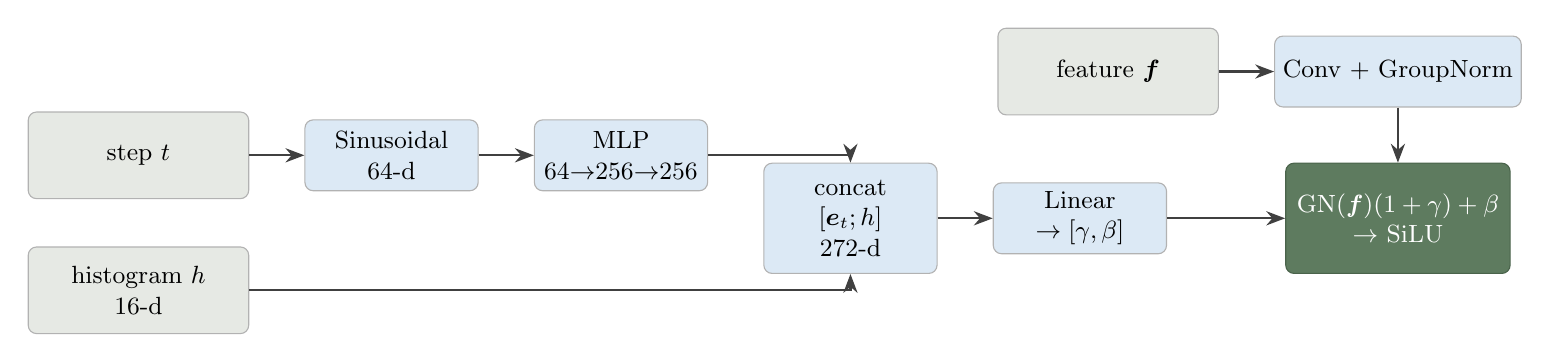
\begin{tikzpicture}[node distance=6mm and 7mm]
\node[lt] (t) {step $t$};
\node[bl, right=of t] (sp) {Sinusoidal\\64-d};
\node[bl, right=of sp] (mlp) {MLP\\$64{\rightarrow}256{\rightarrow}256$};
\node[lt, below=of t] (h) {histogram $h$\\16-d};
\node[bl, right=of mlp, yshift=-8mm, minimum height=14mm] (cat) {concat\\$[\bm e_t;h]$\\272-d};
\node[bl, right=of cat] (lin) {Linear\\$\rightarrow[\gamma,\beta]$};
\node[dk, right=of lin, xshift=8mm, minimum height=14mm] (film) {$\mathrm{GN}(\bm f)(1+\gamma)+\beta$\\$\rightarrow$ SiLU};
\node[bl, above=7mm of film] (gn) {Conv + GroupNorm};
\node[lt, left=of gn] (f) {feature $\bm f$};
\draw[ar] (t)--(sp); \draw[ar] (sp)--(mlp); \draw[ar] (mlp)-|(cat); \draw[ar] (h)-|(cat);
\draw[ar] (cat)--(lin); \draw[ar] (f)--(gn); \draw[ar] (gn)--(film); \draw[ar] (lin)--(film);
\end{tikzpicture}
\end{adjustbox}
\caption{How $t$ and the histogram $h$ condition each ResBlock (FiLM) [code].}
\end{figure}


\textbf{Noise schedule:} cosine, $T=300$ steps:
\begin{equation}
\abar_t=\frac{f(t)}{f(0)},\qquad f(t)=\cos^2\!\Big(\frac{t/T+0.008}{1.008}\cdot\frac{\pi}{2}\Big).
\end{equation}

% =====================================================
\section{Training}\label{sec:train}

\subsection{Inputs, output, loss}
\begin{center}
\small
\begin{tabularx}{\linewidth}{lX}
\toprule
\textbf{Inputs to the network} & noisy patch $\x_t$ (1 channel), time step $t$, histogram $h$ (16 numbers) \\
\textbf{Not an input} & the mask $M_f$ -- it is used only in the loss \\
\textbf{Output} & predicted noise $\hat\eps$ (same size as the patch) \\
\textbf{Loss} & L1 error between real and predicted noise, inside the mask only \\
\bottomrule
\end{tabularx}
\end{center}

\textbf{Add noise:}
\begin{equation}
\x_t=\sqrt{\abar_t}\,\x_0+\sqrt{1-\abar_t}\,\eps,\qquad \eps\sim\N(\bm 0,\I).
\end{equation}
\textbf{Loss (code):}
\begin{equation}
\Loss=\frac{1}{|\Omega|}\sum_{v\in\Omega}\big|M_f(v)\,\epsilon(v)-M_f(v)\,\hat\epsilon(v)\big|,
\end{equation}
where $\Omega$ = all voxels in the batch. Because it divides by \emph{all} voxels, small lesions give small loss values.

\textbf{Histogram (code):} 16 bins over the whole normalised range $[-1,1]$, divided by the number of mask voxels:
\begin{verbatim}
hist = torch.histc(img[mask > 0], bins=16, min=-1, max=1) / mask.sum()
\end{verbatim}

\subsection{Settings in the code}
\begin{center}
\small
\begin{tabular}{ll}
\toprule
\textbf{Setting} & \textbf{Value} \\
\midrule
Patch size & $32\times64\times64$ (depth first), hard-coded in the dataset file \\
Intensity & HU clipped to $[-1000,400]$ (lung), scaled to $[-1,1]$, hard-coded \\
Augmentation & random flip on one axis \\
Steps $T$ & 300, cosine \\
Optimiser & Adam, learning rate $10^{-4}$ \\
Batch & 20, gradient accumulation 2 \\
Training steps & 50{,}001 (README: 20k--50k is enough) \\
EMA & 0.995, every 10 steps, from step 2{,}000 \\
Checkpoints & every 1{,}000 steps: \texttt{model-N.pt} (keys \texttt{model} and \texttt{ema}) \\
Compute (README) & 5$\times$A100 40\,GB, 2.5 days for 50k steps \\
\bottomrule
\end{tabular}
\end{center}

\begin{algorithm}[H]
\caption{One training step}
\begin{algorithmic}[1]
\State Take a lesion patch $\x_0$, its mask $M_f$, its histogram $h$
\State Pick a random step $t$ and random noise $\eps$
\State $\x_t \gets \sqrt{\abar_t}\,\x_0+\sqrt{1-\abar_t}\,\eps$ \Comment{whole patch is noised}
\State $\hat\eps \gets \text{U-Net}(\x_t,t,h)$
\State $\Loss \gets \operatorname{mean}|M_f\had\eps-M_f\had\hat\eps|$
\State Update weights; update EMA copy
\end{algorithmic}
\end{algorithm}

% =====================================================
\section{Inference (generation)}\label{sec:infer}

\subsection{Inputs and output}
\begin{center}
\small
\begin{tabularx}{\linewidth}{lX}
\toprule
\textbf{Inputs} & normal patch $\x^{\text{normal}}$ (no lesion), mask $M_f$ (where to draw), histogram $h$ (how it looks) \\
\textbf{Output} & synthetic patch with a lesion inside $M_f$; the mask $M_f$ is saved with it \\
\bottomrule
\end{tabularx}
\end{center}

\subsection{What happens at each step}
At every step, \emph{first} the outside of the mask is replaced by the real patch (with the right noise), \emph{then} the network takes one denoising step:
\begin{align}
\hat\x_t &= \sqrt{\abar_t}\,\x^{\text{normal}}+\sqrt{1-\abar_t}\,\eps && \text{(real patch, noised)}\\
\x_t &\gets \hat\x_t\had(1-M_f)+\x_t\had M_f && \text{(combine)}\\
\x_{t-1} &= \text{DDPM step from U-Net}(\x_t,t,h) && \text{(denoise whole patch)}
\end{align}

\textbf{Going back and forth (RePaint).} The code sometimes adds noise back, $\x_t=\sqrt{1-\beta_t}\,\x_{t-1}+\sqrt{\beta_t}\,\bm n$, and denoises again, so the lesion blends with its surroundings~\cite{repaint}. Settings: \texttt{jump\_length} and \texttt{jump\_n\_sample} (script: 5 and 5; README: 2--10 works; about 40\,s per patch on an A100 with 2 and 2).

\begin{algorithm}[H]
\caption{Generation (simplified)}
\begin{algorithmic}[1]
\State Inputs: normal patch $\x^{\text{normal}}$, mask $M_f$, histogram $h$
\State $\x_T\sim\N(\bm 0,\I)$
\For{each step in the RePaint schedule}
  \If{going down}
    \State replace outside of $M_f$ with $\sqrt{\abar_t}\,\x^{\text{normal}}+\sqrt{1-\abar_t}\,\eps$
    \State $\x_{t-1}\gets$ one denoising step with U-Net$(\x_t,t,h)$
  \Else\ \ add one step of noise back
  \EndIf
\EndFor
\State \Return $\x_0$ and $M_f$
\end{algorithmic}
\end{algorithm}

\begin{caution}
The last step is a network step, so the final output is from the network \emph{everywhere}, also outside the mask (very close to the real patch, but not identical). \textbf{After generation, put the real background back outside $M_f$.}
\end{caution}

\subsection{Histogram types}
The code loads 3 histograms (cluster centres) from \texttt{hist\_clusters/lidc\_clusters.json} (3 $\times$ 16 numbers). For lung nodules they are roughly ground-glass, part-solid and solid. Each is changed by up to $\pm10\%$ at random. With \texttt{types=3}, every patch is generated 3 times, once per histogram, into folders \texttt{Image\_1..3}, \texttt{Mask\_1..3}.

\textbf{Weights:} inference loads the \texttt{model} weights, not the \texttt{ema} weights.

% =====================================================
\section{Paper vs.\ code}\label{sec:diff}
\begin{center}
\small
\begin{tabularx}{\linewidth}{lXX}
\toprule
\textbf{Topic} & \textbf{Paper says} & \textbf{Code does} \\
\midrule
Histogram & cross-attention & joined to time step, FiLM in the first conv of each ResBlock \\
Loss & $L_2$ inside mask & L1 inside mask, averaged over all voxels \\
Steps & not given & 300, cosine \\
Combine step & after the model step & before each model step; final output is all network \\
Compute & $\approx$3 A100, 1 day & README: 5 A100, 2.5 days \\
\bottomrule
\end{tabularx}
\end{center}

% =====================================================
\section{How we use it for aneurysm CTA}\label{sec:ours}

\subsection{Lung (paper) vs.\ our data}
\begin{center}
\small
\begin{tabularx}{\linewidth}{lXX}
\toprule
 & \textbf{Paper (lung)} & \textbf{Ours (aneurysm CTA)} \\
\midrule
Patch & $32\times64\times64$ around a nodule & $64^3$ at 0.45\,mm around an aneurysm (small random shift) \\
Intensity & $[-1000,400]$ HU & $[-100,900]$ HU \\
Number of patches & 2{,}104 & $\approx$1{,}300 (full data); $\approx$117 now (pilot only) \\
Histogram clusters & lung clusters & make our own 3 clusters from our training histograms \\
Normal patches & healthy lungs & vessel branches $>$15\,mm from any aneurysm \\
Masks at generation & real or DiffMask & shape library (real shapes, resized, rotated, placed on the vessel wall) \\
\bottomrule
\end{tabularx}
\end{center}

\subsection{Folders and file names (required by the code)}
\begin{verbatim}
data/AneurysmCTA/
  Pathological/                      <- training
    Image/  Tr0001_Vol_01.nii.gz      (aneurysm patch)
    Mask/   Tr0001_Mask_01.nii.gz     ("Vol_" -> "Mask_")
    test.txt                          (names to EXCLUDE, no .nii.gz)
  Normal/                            <- generation
    Image/  Tr0123_CVol_01.nii.gz     (normal vessel patch; must contain "_CVol_")
    Mask/   Tr0123_CMask_01.nii.gz    (placed mask)
\end{verbatim}
\begin{itemize}
  \item The mask is found by replacing \texttt{Vol\_} with \texttt{Mask\_} in the file name.
  \item Generation splits the name at \texttt{\_CVol\_}; without it, saving crashes.
  \item \texttt{test.txt} lists validation patches that are left out (it is also applied during generation).
\end{itemize}

\subsection{Code changes}
\textbf{1. Intensity window and patch size} -- in \emph{both} \texttt{LeFusion/dataset/lidc\_hist.py} and \texttt{lidc\_hist\_in.py}:
\begin{verbatim}
tio.Clamp(out_min=-100, out_max=900)
tio.RescaleIntensity(in_min_max=(-100, 900), out_min_max=(-1.0, 1.0))
tio.CropOrPad(target_shape=(64, 64, 64))     # image AND mask transforms
\end{verbatim}
\textbf{2. Depth} -- set \texttt{diffusion\_depth\_size=64} in the train and inference scripts. Depth is never made smaller in the U-Net, so memory is about $2\times$ the paper's: use batch 4--8.

\textbf{3. Histogram clusters} -- make \texttt{hist\_clusters/lidc\_clusters.json} from our data: run k-means ($k=3$) on our training histograms (low / medium / high contrast). Same format: \texttt{[\{"n\_class": 3, "centers": [[16 numbers], ...]\}]}.

\textbf{4. Smaller fixes}
\begin{itemize}
  \item \texttt{lidc\_train.sh}: \texttt{results\_folder} points to \texttt{EMIDEC}; set your own folder.
  \item \texttt{num\_workers} is 20 by default; use 2--4 on Colab or Kaggle.
  \item Install from the repo root (\texttt{pip install -r requirements.txt}); the README's \texttt{LeFusion\_LIDC} folder does not exist.
  \item Optional: load \texttt{ema} weights at inference; average the loss over mask voxels only; give the mask as a 2nd input channel (bigger change).
\end{itemize}

\subsection{Training flow}
\begin{figure}[H]
\centering
\begin{adjustbox}{max width=\linewidth}
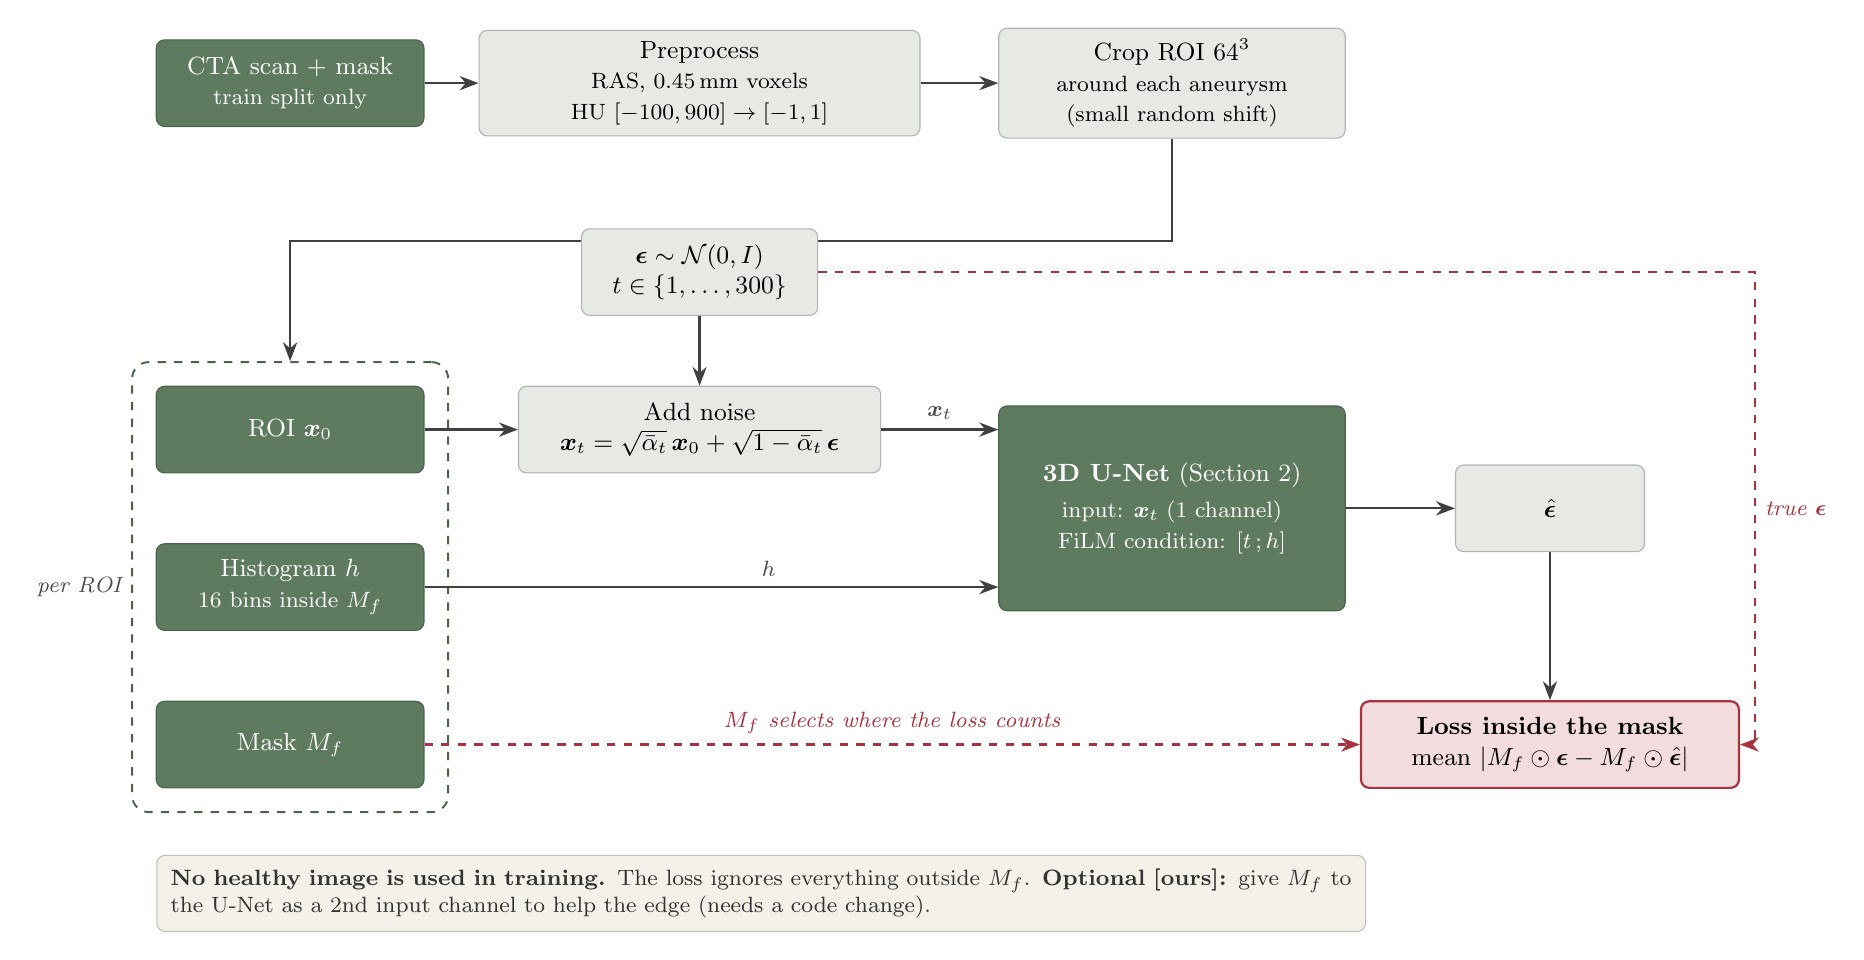
\begin{tikzpicture}[x=1mm,y=1mm]
% row 1: data prep
\node[dk, minimum width=34mm] (scan) at (0,14) {CTA scan + mask\\\footnotesize train split only};
\node[lt, minimum width=56mm] (pre) at (52,14) {Preprocess\\\footnotesize RAS, 0.45\,mm voxels\\\footnotesize HU $[-100,900]\rightarrow[-1,1]$};
\node[lt, minimum width=44mm] (crop) at (112,14) {Crop ROI $64^3$\\\footnotesize around each aneurysm\\\footnotesize (small random shift)};
\draw[ar] (scan)--(pre); \draw[ar] (pre)--(crop);
% inputs
\node[dk, minimum width=34mm] (x0) at (0,-30) {ROI $\x_0$};
\node[dk, minimum width=34mm] (h) at (0,-50) {Histogram $h$\\\footnotesize 16 bins inside $M_f$};
\node[dk, minimum width=34mm] (mf) at (0,-70) {Mask $M_f$};
\begin{scope}[on background layer]\node[frame, fit=(x0)(h)(mf), inner sep=3mm, label={[lb]left:per ROI}] (inp) {};\end{scope}
\draw[ar] (crop.south) |- (0,-6) -- (inp.north);
% noise + net
\node[lt, minimum width=30mm] (eps) at (52,-10) {$\eps\sim\N(0,I)$\\$t\in\{1,\dots,300\}$};
\node[lt, minimum width=46mm] (nz) at (52,-30) {Add noise\\$\x_t=\sqrt{\abar_t}\,\x_0+\sqrt{1-\abar_t}\,\eps$};
\node[dk, minimum width=44mm, minimum height=26mm] (u) at (112,-40) {\textbf{3D U-Net} (Section 2)\\[2pt]\footnotesize input: $\x_t$ (1 channel)\\\footnotesize FiLM condition: $[t\,;h]$};
\node[lt, minimum width=24mm] (eh) at (160,-40) {$\hat\eps$};
\node[ls, minimum width=48mm] (loss) at (160,-70) {\textbf{Loss inside the mask}\\$\operatorname{mean}\,|M_f\odot\eps-M_f\odot\hat\eps|$};
\draw[ar] (x0)--(nz); \draw[ar] (eps)--(nz);
\draw[ar] (nz.east) -- node[lb,above]{$\x_t$} (nz.east -| u.west);
\draw[ar] (h.east) -- node[lb,above,pos=0.6]{$h$} (h.east -| u.west);
\draw[ar] (u)--(eh); \draw[ar] (eh)--(loss);
\draw[ard] (mf.east) -- node[lb,above,text=rloss,pos=0.5]{$M_f$ selects where the loss counts} (loss.west);
\draw[ard] (eps.east) -- (186,-10) |- node[lb,pos=0.25,right,text=rloss]{true $\eps$} (loss.east);
% note
\node[nt, text width=150mm, anchor=north west] at (-17,-84) {\textbf{No healthy image is used in training.} The loss ignores everything outside $M_f$. \textbf{Optional [ours]:} give $M_f$ to the U-Net as a 2nd input channel to help the edge (needs a code change).};
\end{tikzpicture}
\end{adjustbox}
\caption{Our training flow. Only real aneurysm ROIs, their masks and their histograms are used.}
\end{figure}


\subsection{Generation flow}
\begin{figure}[H]
\centering
\begin{adjustbox}{max width=\linewidth}
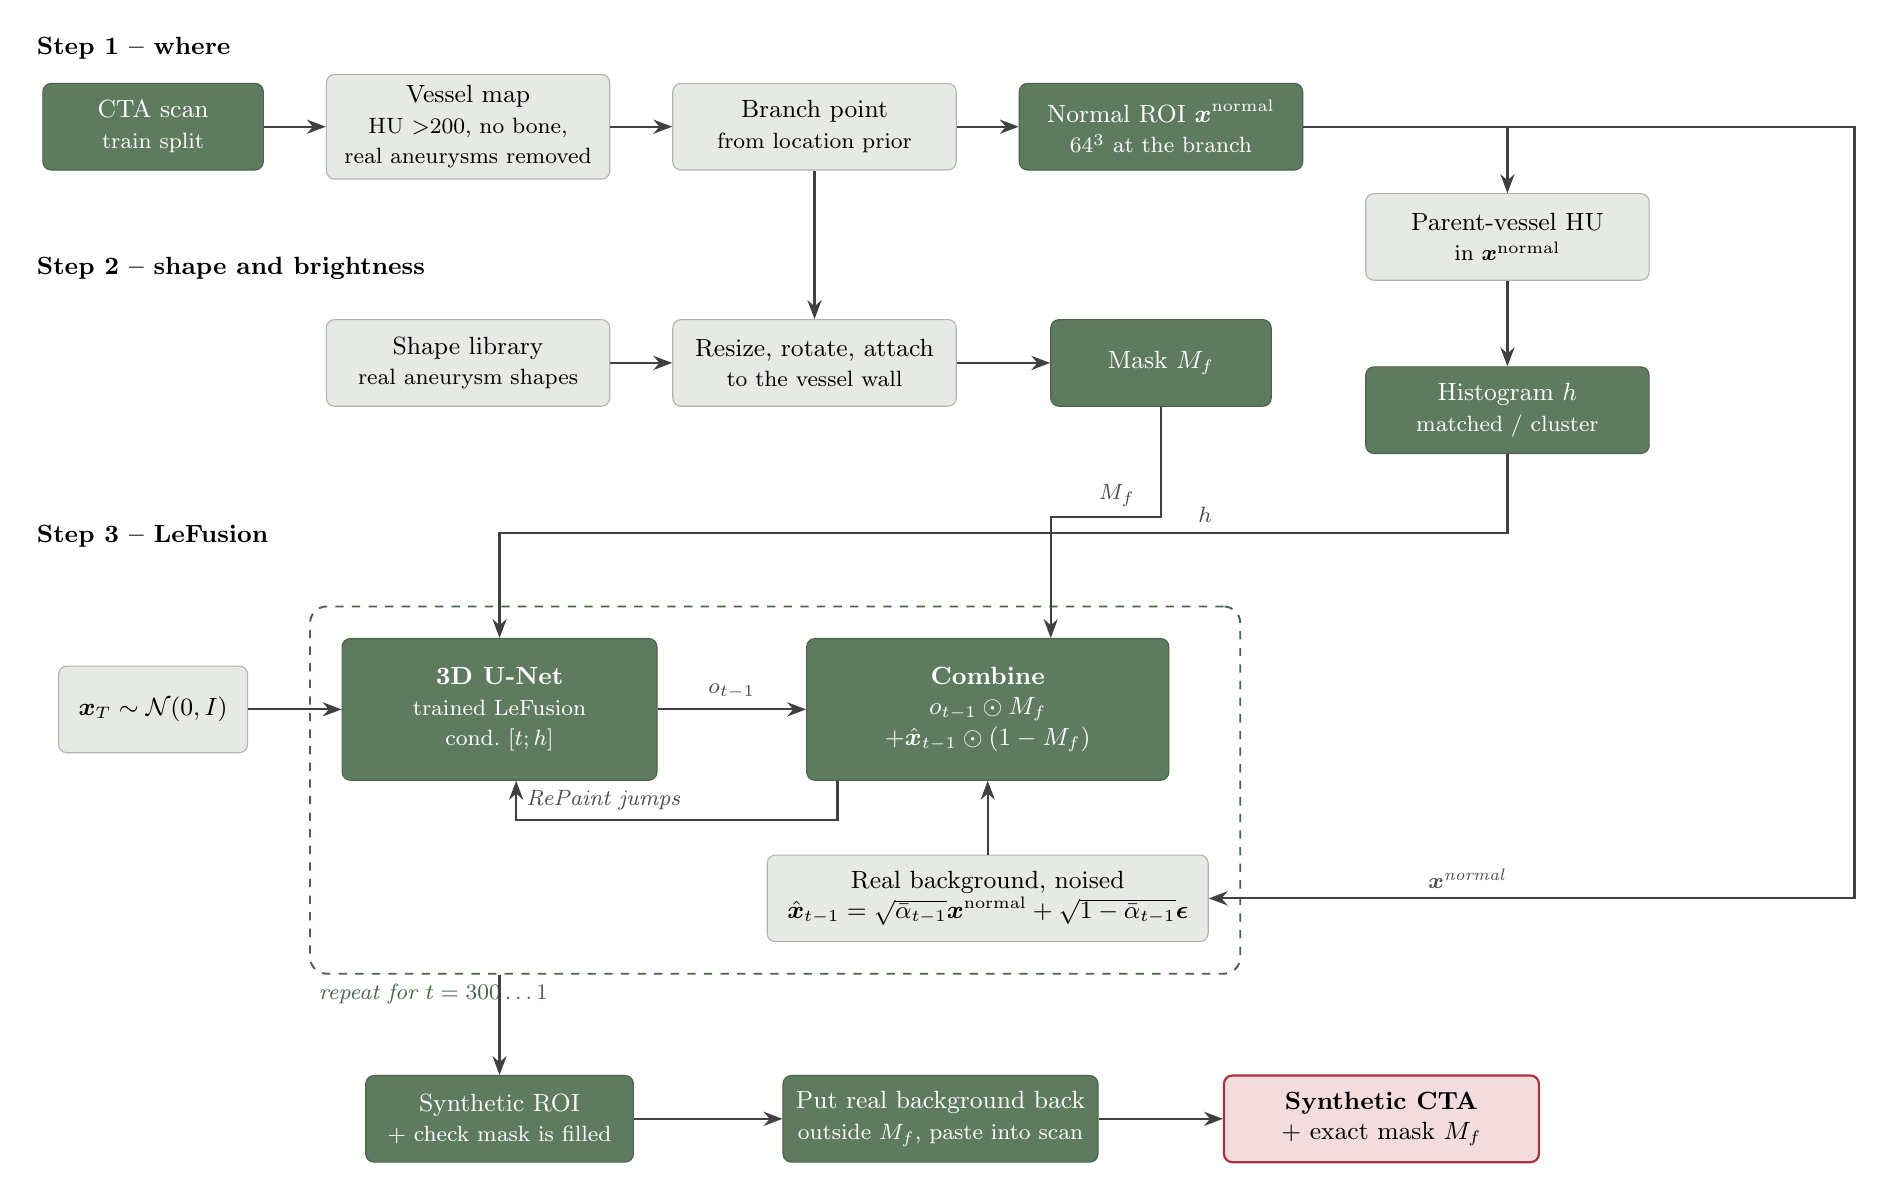
\begin{tikzpicture}[x=1mm,y=1mm]
% step 1
\node[font=\small\bfseries, anchor=west] at (-16,10) {Step 1 -- where};
\node[dk, minimum width=28mm] (scan) at (0,0) {CTA scan\\\footnotesize train split};
\node[lt, minimum width=36mm] (ves) at (40,0) {Vessel map\\\footnotesize HU $>$200, no bone,\\\footnotesize real aneurysms removed};
\node[lt, minimum width=36mm] (br) at (84,0) {Branch point\\\footnotesize from location prior};
\node[dk, minimum width=36mm] (vp) at (128,0) {Normal ROI $\x^{\text{normal}}$\\\footnotesize $64^3$ at the branch};
\draw[ar] (scan)--(ves); \draw[ar] (ves)--(br); \draw[ar] (br)--(vp);
% step 2
\node[font=\small\bfseries, anchor=west] at (-16,-18) {Step 2 -- shape and brightness};
\node[lt, minimum width=36mm] (lib) at (40,-30) {Shape library\\\footnotesize real aneurysm shapes};
\node[lt, minimum width=36mm] (place) at (84,-30) {Resize, rotate, attach\\\footnotesize to the vessel wall};
\node[dk, minimum width=28mm] (mf) at (128,-30) {Mask $M_f$};
\node[lt, minimum width=36mm] (pv) at (172,-14) {Parent-vessel HU\\\footnotesize in $\x^{\text{normal}}$};
\node[dk, minimum width=36mm] (h) at (172,-36) {Histogram $h$\\\footnotesize matched / cluster};
\draw[ar] (lib)--(place); \draw[ar] (place)--(mf); \draw[ar] (br.south) -- (place.north);
\draw[ar] (vp.east) -| (pv.north); \draw[ar] (pv)--(h);
% step 3
\node[font=\small\bfseries, anchor=west] at (-16,-52) {Step 3 -- LeFusion};
\node[lt, minimum width=24mm] (xT) at (0,-74) {$\x_T\sim\N(0,I)$};
\node[dk, minimum width=40mm, minimum height=18mm] (u) at (44,-74) {\textbf{3D U-Net}\\\footnotesize trained LeFusion\\\footnotesize cond.\ $[t;h]$};
\node[dk, minimum width=46mm, minimum height=18mm] (cb) at (106,-74) {\textbf{Combine}\\$o_{t-1}\odot M_f$\\$+\hat\x_{t-1}\odot(1-M_f)$};
\node[lt, minimum width=56mm] (bg) at (106,-98) {Real background, noised\\$\hat\x_{t-1}=\sqrt{\abar_{t-1}}\x^{\text{normal}}+\sqrt{1-\abar_{t-1}}\eps$};
\draw[ar] (xT)--(u); \draw[ar] (u)--node[lb,above]{$o_{t-1}$}(cb); \draw[ar] (bg)--(cb);
\draw[ar] (cb.south west) ++(4,0) |- ++(0,-5) -| node[lb,pos=0.75,right]{RePaint jumps} ([xshift=6]u.south);
\begin{scope}[on background layer]\node[frame, fit=(u)(cb)(bg), inner sep=4mm] (loop) {};\end{scope}
\node[lb, anchor=north west, text=gbord] at (loop.south west) {repeat for $t=300\dots1$};
\draw[ar] (mf.south) -- ++(0,-14) -| node[lb,pos=0.2,above]{$M_f$} ([xshift=8mm]cb.north);
\draw[ar] (h.south) -- ++(0,-10) -| node[lb,pos=0.15,above]{$h$} (u.north);
\draw[ar] (vp.east) -- ++(70,0) |- node[lb,pos=0.8,above]{$\x^{\text{normal}}$} (bg.east);
% output
\node[dk, minimum width=34mm] (o1) at (44,-126) {Synthetic ROI\\\footnotesize + check mask is filled};
\node[dk, minimum width=40mm] (o2) at (100,-126) {Put real background back\\\footnotesize outside $M_f$, paste into scan};
\node[ls, minimum width=40mm] (o3) at (156,-126) {\textbf{Synthetic CTA}\\+ exact mask $M_f$};
\draw[ar] (loop.south -| o1) -- (o1); \draw[ar] (o1)--(o2); \draw[ar] (o2)--(o3);
\end{tikzpicture}
\end{adjustbox}
\caption{Our inference flow without DiffMask. The mask comes from the shape library; the histogram is matched to the parent vessel or taken from one of our 3 clusters.}
\end{figure}


\subsection{Commands}
\textbf{Train:}
\begin{verbatim}
python LeFusion/train/train.py dataset=lidc \
  model.diffusion_img_size=64 model.diffusion_depth_size=64 \
  model.diffusion_num_channels=1 model.cond_dim=16 \
  model.batch_size=6 model.train_num_steps=50001 \
  dataset.root_dir=data/AneurysmCTA/Pathological/Image \
  dataset.test_txt_dir=data/AneurysmCTA/Pathological/test.txt \
  model.results_folder=LeFusion/LeFusion_Model/CTA
\end{verbatim}
\textbf{Generate:}
\begin{verbatim}
python LeFusion/inference/inference.py data_type=lidc types=3 \
  diffusion_img_size=64 diffusion_depth_size=64 diffusion_num_channels=1 \
  batch_size=3 cond_dim=16 \
  test_txt_dir=data/AneurysmCTA/Pathological/test.txt \
  dataset_root_dir=data/AneurysmCTA/Normal/Image/ \
  target_img_path=data/AneurysmCTA/gen/Image/ \
  target_label_path=data/AneurysmCTA/gen/Mask/ \
  model_path=LeFusion/LeFusion_Model/CTA/model-50.pt \
  schedule_jump_params.jump_length=5 schedule_jump_params.jump_n_sample=5
\end{verbatim}
(\texttt{dataset=lidc} / \texttt{data\_type=lidc} just chooses the LIDC code path, which we edited.)

\subsection{Checks}
\begin{itemize}
  \item \textbf{Is the mask filled?} Inside $M_f$, at least 70\% of voxels should be bright (HU $>$ 200). If not, reject the sample.
  \item \textbf{Look} at 30--50 samples: the aneurysm should grow from the vessel, with no seam.
  \item \textbf{Brightness:} compare HU inside synthetic vs.\ real aneurysms.
  \item \textbf{No copying:} no sample should be almost the same as a training patch.
  \item \textbf{Real test:} nnU-Net trained on real vs.\ real + synthetic, tested on real scans only.
\end{itemize}

\begin{caution}
With 99 scans ($\approx$117 aneurysms) the model will likely copy training examples -- use it only to test the pipeline. Leaving the lung window in the code is the easiest mistake to miss.
\end{caution}

\begin{thebibliography}{9}\small
\bibitem{lefusion} H.~Zhang, Y.~Liu, J.~Yang, S.~Wan, X.~Wang, W.~Peng, P.~Fua. LeFusion: Controllable pathology synthesis via lesion-focused diffusion models. \emph{ICLR}, 2025. arXiv:2403.14066.
\bibitem{repaint} A.~Lugmayr, M.~Danelljan, A.~Romero, F.~Yu, R.~Timofte, L.~Van~Gool. RePaint: Inpainting using denoising diffusion probabilistic models. \emph{CVPR}, 2022.
\end{thebibliography}

\end{document}
